\section{Appendix}

\crefalias{section}{appsec}
\newpage

\begin{landscape}
    \subsection{Literature on Trade Classification Using Machine Learning}
    \label{app:literature-ml-tc}
    \begin{table}[ht]
        \centering
        \caption[Literature on Trade Classification Using Machine Learning.]{Literature on trade classification using machine learning. Improvement is the out-of-sample performance over the best baselines if multiple baselines are reported. Data requirements may not be identical to these of classical rules.}
        \label{tab:literature-trade-classification-ml}
        \begin{tabular}{@{}p{3cm}p{3cm}lp{4cm}p{4cm}l@{}}
            \toprule
            Research                                                                & Data                              & Sample Period            & Method                                                                                                & Baseline                                                     & Improvement              \\ \midrule
            \autocite[][411]{rosenthalModelingTradeDirection2012}         & \gls{NASDAQ}                      &                          & Logistic regression                                                                                   & \gls{EMO} rule, \gls{LR} rule,\newline and tick rule         & max. \SI{2.2}{\percent}  \\ \cmidrule{2-6}
                                                                                    & \gls{NYSE}                        & 03/12/2004 -- 31/12/2004 & Logistic regression                                                                                   & \gls{EMO} rule, \gls{LR} rule,\newline and tick rule         & max. \SI{1.1}{\percent}  \\\cmidrule{1-6}
            \autocite[][489--493]{blazejewskiLocalNonParametricModel2005} & Australian Stock\newline Exchange & 11/11/2002 -- 27/08/2003 & $k$ nearest neighbor, \newline logistic regression,\newline trade continuation,\newline majority vote & -                                                            & -                        \\ \cmidrule{1-6}
            \autocite[][49--57]{ronenMachineLearningTrade2022}            & \gls{TRACE}                       & 01/07/2002 -- 31/12/2019 & Logistic regression, decision tree,\newline neural network, and random forests                        & \gls{LR} rule and tick rule,\newline and \gls{BVC} algorithm & max. \SI{13.3}{\percent} \\ \cmidrule{2-6}
                                                                                    & \gls{NASDAQ}                      & 09/12/2013 -- 13/12/2013 & Logistic regression, decision tree,\newline neural network, and random forests                        & \gls{LR} rule, tick rule,\newline and \gls{BVC} algorithm    & max. \SI{3.3}{\percent}  \\ \bottomrule
        \end{tabular}
    \end{table}
\end{landscape}

\subsection{Summary Statistics}
\label{app:summary-statistics}

\begin{table}[ht]
    \centering
    \sisetup{table-format=4.2,table-alignment-mode = none, table-number-alignment=left, table-text-alignment = left}
    \caption[Summary Statistics for \glsshortkey{ISE} Sample]{Summary statistics for \gls{ISE} labelled sample. Time to maturity in months.}
    \label{tab:ise-supervised-all}
    \begin{tabular}{@{}lSSSSSSSSS@{}}
        \toprule
        {}               & {Mean}     & {SD}        & {1\%}    & {5\%}    & {25\%}    & {Median}  & {75\%}     & {95\%}      & {99\%}      \\
        \midrule
        trade price      & 4.975898   & 15.722798   & 0.010000 & 0.050000 & 0.460000  & 1.540000  & 4.300000   & 17.799999   & 59.200001   \\
        bid (ex)         & 4.831530   & 15.563911   & 0.000000 & 0.010000 & 0.400000  & 1.450000  & 4.150000   & 17.400000   & 58.400002   \\
        ask (ex)         & 5.144752   & 15.946395   & 0.020000 & 0.070000 & 0.520000  & 1.650000  & 4.500000   & 18.299999   & 60.400002   \\
        ask (best)       & 5.150689   & 101.225182  & 0.020000 & 0.060000 & 0.500000  & 1.600000  & 4.500000   & 18.100000   & 60.000000   \\
        bid (best)       & 4.849738   & 15.569823   & 0.000000 & 0.020000 & 0.400000  & 1.450000  & 4.200000   & 17.400000   & 58.400002   \\
        price lag (ex)   & 5.009203   & 15.326354   & 0.020000 & 0.080000 & 0.550000  & 1.630000  & 4.400000   & 17.750000   & 59.000000   \\
        price lead (ex)  & 5.035194   & 15.649212   & 0.020000 & 0.060000 & 0.500000  & 1.600000  & 4.400000   & 17.990000   & 59.759998   \\
        price lag (all)  & 4.962591   & 15.660495   & 0.020000 & 0.060000 & 0.500000  & 1.550000  & 4.300000   & 17.680000   & 58.860001   \\
        price lead (all) & 5.005602   & 21.510473   & 0.020000 & 0.050000 & 0.500000  & 1.570000  & 4.350000   & 17.879999   & 59.200001   \\\addlinespace
        trade size       & 13.615033  & 77.752615   & 1.000000 & 1.000000 & 1.000000  & 4.000000  & 10.000000  & 50.000000   & 150.000000  \\
        bid size (ex)    & 266.541321 & 1112.201294 & 0.000000 & 1.000000 & 20.000000 & 57.000000 & 197.000000 & 1092.000000 & 2995.000000 \\
        ask size (ex)    & 280.400757 & 1184.970825 & 1.000000 & 2.000000 & 21.000000 & 63.000000 & 214.000000 & 1121.000000 & 3029.000000 \\\addlinespace
        strike price     & 110.803169 & 350.870270  & 4.000000 & 9.000000 & 25.000000 & 45.000000 & 85.000000  & 310.000000  & 1260.000000 \\
        ttm              & 3.430495   & 4.930164    & 0.000000 & 0.000000 & 1.000000  & 1.000000  & 4.000000   & 15.000000   & 24.000000   \\
        moneyness        & 7.000215   & 2299.693359 & 0.476429 & 0.685166 & 0.884600  & 0.967481  & 1.038636   & 1.290323    & 1.824375    \\
        \bottomrule
    \end{tabular}
\end{table}




\clearpage

\subsection{Power-Transforms of Features}
\label{app:power-transforms-of-features}

\begin{table}[ht]
    \centering
    \caption[Power-Transforms of Features]{Power-transforms of features. \lambda~specifies the exponent. Transformations estimated on \gls{ISE} training set.}
    \label{tab:power-transformerations}
    \begin{tabular}{lS}
        \toprule
        {Feature}        & {\lambda} \\
        \midrule
        strike price     & -0.082968 \\
        trade size       & -0.204893 \\
        trade price      & 0.060425  \\
        bid (best)       & 0.110299  \\
        ask (best)       & 0.056837  \\
        ask (ex)         & 0.049090  \\
        bid (ex)         & 0.113067  \\
        bid size (ex)    & 0.140284  \\
        ask size (ex)    & 0.029876  \\
        price lead (all) & 0.054975  \\
        price lag (all)  & 0.049097  \\
        price lead (ex)  & 0.053774  \\
        price lag (ex)   & 0.042910  \\
        day volume       & -0.116017 \\
        moneyness        & -0.109716 \\
        \bottomrule
    \end{tabular}
\end{table}

\subsection{Features and Transformations}
\label{app:feature-and-transformations}

\begin{table}[H]
    \centering
    \begin{threeparttable}
        \begin{tabular}{@{}ll@{}}
            \toprule
            Feature Name            & Transform              \\ \midrule
            trade price             & $\log$ + standardized  \\
            price lag (ex)          & $\log$ + standardized  \\
            price lag (all)         & $\log$ + standardized  \\
            price change lag (ex)   & clipped + standardized \\
            price change lag (all)  & clipped + standardized \\
            price lead (ex)         & $\log$ + standardized  \\
            price lead (all)        & $\log$ + standardized  \\
            price change lead (ex)  & clipped + standardized \\
            price change lead (all) & clipped + standardized \\
            bid (best)              & $\log$ + standardized  \\
            bid (ex)                & $\log$ + standardized  \\
            ask (best)              & $\log$ + standardized  \\
            ask (ex)                & $\log$ + standardized  \\
            prox. to quotes (ex)    & clipped + standardized \\
            prox. to quotes (best)  & clipped + standardized \\ \addlinespace
            bid ask size ratio (ex) & clipped + standardized \\
            bid size (ex)           & $\log$ + standardized  \\
            ask size (ex)           & $\log$ + standardized  \\
            rel. bid size (ex)      & clipped + standardized \\
            rel. ask size (ex)      & clipped + standardized \\
            trade size              & $\log$ + standardized  \\ \addlinespace
            strike price            & $\log$ + standardized  \\
            volume option series    & $\log$ + standardized  \\ 
            root                    & binarised              \\ 
            time to maturity        & standardized           \\
            moneyness               & standardized           \\
            option type             & binarised              \\
            issue type              & binarised              \\ \bottomrule
        \end{tabular}
        \begin{tablenotes}\footnotesize
            \item[*] Notation assumes, that the previous or next trade price is distinguishable.
        \end{tablenotes}
    \end{threeparttable}
    \caption[Overview of Features and Transformations]{Overview of features and transformations.}
    \label{tab:features-transformations}
\end{table}

\newpage
\subsection{Autocorrelation of Features}
\label{app:autocorrelation-of-features}

\begin{figure}[ht]
    \centering
    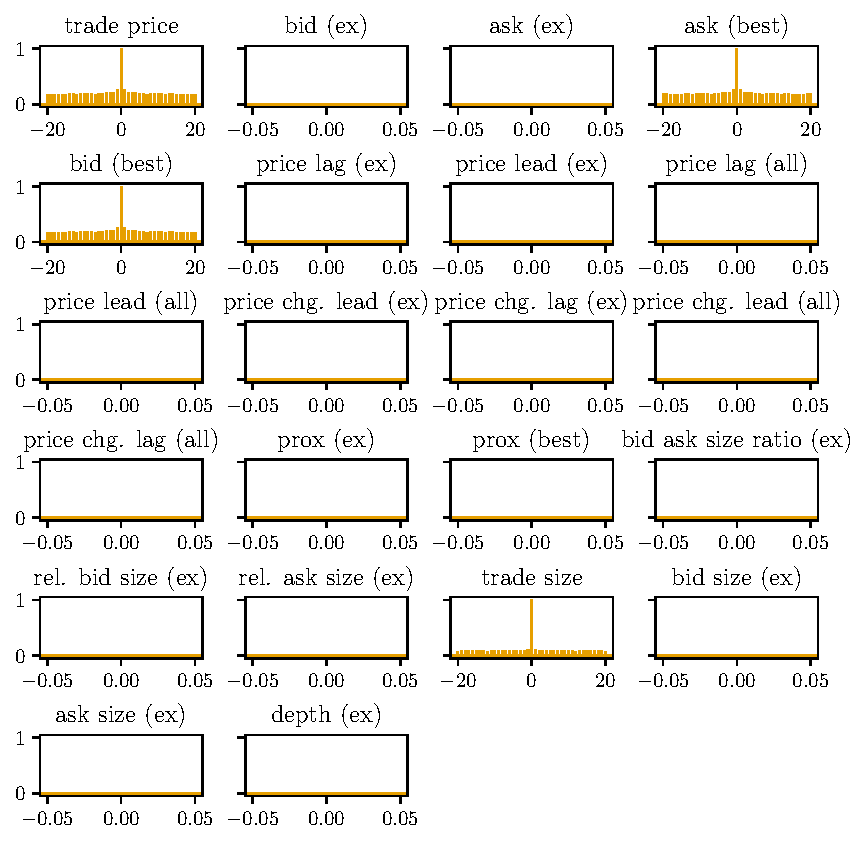
\includegraphics{auto_corr_features.pdf}
    \caption[Autocorrelation of Features]{Autocorrelation of features.}
    \label{fig:auto-correlation-features}
\end{figure}

\newpage
\subsection{Results of Supervised Models With Re-training}
\label{app:results-of-supervised-models-with-re-training}

\begin{table}[ht]
    \centering
    \caption[Accuracies of Supervised Approaches With Re-Training On \glsentryshort{CBOE} and \glsentryshort{ISE}]{This table reports the accuracy of \glspl{GBRT} for different feature sets on the \gls{ISE} and \gls{CBOE} test set after re-training on \gls{ISE} training and validation set. The absolute improvements over \gls{GSU} (small) for the feature set classic and \gls{GSU} (large) for all other feature sets are given in the +/- column.}
    \label{tab:results-supervised-retraining-ise-cboe}
    \begin{tabular}{@{}llSSSSSS@{}}
        \toprule
                   &            & \multicolumn{2}{c}{\gls{FS} Classical} & \multicolumn{2}{c}{\gls{FS} Size} & \multicolumn{2}{c}{\gls{FS} Option}                                      \\ \cmidrule(lr){3-4}\cmidrule(lr){5-6} \cmidrule(lr){7-8}
        Classifier & Data Set   & {Acc. in \%}                           & {+/-}                             & {Acc. in \%}                        & {+/-}    & {Acc. in \%} & {+/-}    \\ \midrule
        \gls{GBRT} & \gls{ISE}  & 66.413827                              & 6.360000                          & 73.945544                           & 6.330000 & 76.162269    & 8.550000 \\
                   & \gls{CBOE} & 67.526839                              & 6.780000                          & 72.754664                           & 6.240000 & 75.125406    & 8.610000 \\ \bottomrule
    \end{tabular}
\end{table}

\newpage
\subsection{Robustness of Gradient Boosting With Self-Training}
\label{app:robustness-of-gradient-boosting-with-self-training}

\begin{table}
    \centering
    \caption[Robustness of Gradient Boosting With Self-Training on \glsentryshort{ISE}]{Accuracies of the \gls{GBRT} with self-training across all sub-samples of the \gls{ISE} test set over time and by proximity to quotes, as well as option characteristics such as option and security type, time to maturity in days, and moneyness. The security type category "Others" encompasses options written on \glspl{ETF}, mutual funds, and \glspl{ADR}. The absolute improvements over \gls{GSU} (small) for the feature set classic and \gls{GSU} (large) for all other feature sets are given in the +/- column.}
    \label{tab:diff-ise-gbm-semi}
    \begin{tabular}{lSSSSSS@{}}
        \toprule
        {}                          & \multicolumn{2}{c}{\glsentryshort{FS} Classic} & \multicolumn{2}{c}{\glsentryshort{FS} Size} & \multicolumn{2}{c}{\glsentryshort{FS} Option}                                        \\ \cmidrule(lr){2-3}\cmidrule(lr){4-5}\cmidrule(lr){6-7}
        {}                          & {Acc. in \%}                                   & {+/-}                                       & {Acc. in \%}                                  & {+/-}     & {Acc. in \%} & {+/-}     \\\midrule
        \multicolumn{7}{l}{ Option Type}                                                                                                                                                                                  \\
        \tabindent Call             & 62.652675                                      & 3.480000                                    & 71.692310                                     & 4.280000  & 73.080774    & 5.670000  \\
        \tabindent Put              & 64.248224                                      & 3.190000                                    & 72.686646                                     & 4.840000  & 74.057310    & 6.210000  \\
        \cmidrule(rl){1-7}
        \multicolumn{7}{l}{ Security Type}                                                                                                                                                                                \\
        \tabindent Index option     & 55.804436                                      & -2.000000                                   & 56.841230                                     & -1.660000 & 57.069948    & -1.430000 \\
        \tabindent Others           & 68.063622                                      & 2.540000                                    & 76.242209                                     & 5.660000  & 77.167487    & 6.590000  \\
        \tabindent Stock option     & 61.635859                                      & 3.750000                                    & 70.742796                                     & 4.190000  & 72.323667    & 5.770000  \\
        \cmidrule(rl){1-7}
        \multicolumn{7}{l}{Trade Size}                                                                                                                                                                                    \\
        \tabindent 1 contract       & 61.639494                                      & 3.100000                                    & 72.340844                                     & 3.170000  & 73.654797    & 4.480000  \\
        \tabindent (1,3] contracts  & 62.223821                                      & 3.770000                                    & 72.789348                                     & 3.500000  & 74.255320    & 4.970000  \\
        \tabindent (3,5] contracts  & 62.397287                                      & 3.590000                                    & 72.519880                                     & 3.120000  & 74.039560    & 4.640000  \\
        \tabindent (5,11] contracts & 65.618460                                      & 3.070000                                    & 71.684199                                     & 8.020000  & 73.028391    & 9.360000  \\
        \tabindent >11 contracts    & 67.040031                                      & 3.370000                                    & 71.118780                                     & 6.160000  & 72.439817    & 7.480000  \\
        \cmidrule(rl){1-7}
        \multicolumn{7}{l}{ Year}                                                                                                                                                                                         \\
        \tabindent 2015             & 60.243706                                      & 3.840000                                    & 68.868343                                     & 5.080000  & 70.786068    & 7.000000  \\
        \tabindent 2016             & 63.512307                                      & 3.340000                                    & 72.378496                                     & 4.860000  & 73.722111    & 6.200000  \\
        \tabindent 2017             & 64.193287                                      & 3.200000                                    & 72.748578                                     & 3.650000  & 74.032503    & 4.930000  \\
        \cmidrule(rl){1-7}
        \multicolumn{7}{l}{ Time To Maturity}                                                                                                                                                                             \\
        \tabindent <= 1 month       & 64.191702                                      & 3.310000                                    & 72.575096                                     & 5.060000  & 73.992504    & 6.480000  \\
        \tabindent (1-2] months     & 64.304365                                      & 3.490000                                    & 72.671822                                     & 4.100000  & 73.423384    & 4.850000  \\
        \tabindent (2-3] months     & 62.723994                                      & 2.820000                                    & 71.532663                                     & 3.250000  & 72.521370    & 4.240000  \\
        \tabindent (3-6] months     & 61.580416                                      & 3.440000                                    & 71.045351                                     & 3.180000  & 72.269140    & 4.410000  \\
        \tabindent (6-12] months    & 61.499195                                      & 3.580000                                    & 71.030021                                     & 3.140000  & 72.522064    & 4.630000  \\
        \tabindent > 12 months      & 54.968983                                      & 3.680000                                    & 68.438668                                     & 3.410000  & 71.434925    & 6.410000  \\
        \cmidrule(rl){1-7}
        \multicolumn{7}{l}{ Moneyness}                                                                                                                                                                                    \\
        \tabindent <= 0.7           & 65.208146                                      & 3.470000                                    & 72.054059                                     & 7.660000  & 72.305804    & 7.910000  \\
        \tabindent (0.7-0.9]        & 67.296529                                      & 3.330000                                    & 74.095772                                     & 5.800000  & 74.898137    & 6.610000  \\
        \tabindent (0.9-1.1]        & 63.795656                                      & 3.270000                                    & 72.767171                                     & 4.190000  & 73.884687    & 5.310000  \\
        \tabindent (1.1-1.3]        & 54.138334                                      & 3.890000                                    & 66.047839                                     & 4.020000  & 69.444851    & 7.420000  \\
        \tabindent > 1.3            & 52.429063                                      & 3.580000                                    & 62.764020                                     & 2.550000  & 69.521397    & 9.310000  \\
        \cmidrule(rl){1-7}
        \multicolumn{7}{l}{ Proximity To Quotes}                                                                                                                                                                          \\
        \tabindent  At mid          & 62.504158                                      & 5.350000                                    & 72.020690                                     & 3.870000  & 74.135598    & 5.990000  \\
        \tabindent  Inside          & 62.254246                                      & 1.810000                                    & 68.066336                                     & 3.560000  & 69.616667    & 5.110000  \\
        \tabindent  At Quotes       & 67.774587                                      & 7.810000                                    & 86.631144                                     & 8.420000  & 87.044176    & 8.830000  \\
        \tabindent  Outside         & 60.665638                                      & -6.110000                                   & 61.222573                                     & -3.700000 & 63.007448    & -1.910000 \\
        \tabindent  Unknown         & 78.419432                                      & 2.010000                                    & 78.173110                                     & 1.770000  & 78.775231    & 2.370000  \\
        \cmidrule(rl){1-7}
        All                         & 63.397514                                      & 3.350000                                    & 72.156489                                     & 4.550000  & 73.536644    & 5.930000  \\
        \bottomrule
    \end{tabular}
\end{table}

\begin{table}[!ht]
    \centering
    \caption[Robustness of Gradient Boosting With Self-Training on \glsentryshort{CBOE}]{Accuracies of the \gls{GBRT} with self-training across all sub-samples of the \gls{CBOE} test set over time and by proximity to quotes, as well as option characteristics such as option and security type, time to maturity in days, and moneyness. The security type category "Others" encompasses options written on \glspl{ETF}, mutual funds, and \glspl{ADR}. The absolute improvements over \gls{GSU} (small) for the feature set classic and \gls{GSU} (large) for all other feature sets are given in the +/- column.}
    \label{tab:diff-cboe-gbm-semi}
    \begin{tabular}{lSSSSSS@{}}
        \toprule
        {}                           & \multicolumn{2}{c}{\glsentryshort{FS} Classic} & \multicolumn{2}{c}{\glsentryshort{FS} Size} & \multicolumn{2}{c}{\glsentryshort{FS} Option}                                        \\ \cmidrule(lr){2-3}\cmidrule(lr){4-5}\cmidrule(lr){6-7}
        {}                           & {Acc. in \%}                                   & {+/-}                                       & {Acc. in \%}                                  & {+/-}     & {Acc. in \%} & {+/-}     \\\midrule
        \multicolumn{7}{l}{ Option Type}                                                                                                                                                                                   \\
        \tabindent  Call             & 65.684960                                      & 5.550000                                    & 71.679647                                     & 5.740000  & 73.861831    & 7.930000  \\
        \tabindent  Put              & 66.793889                                      & 5.310000                                    & 72.213858                                     & 5.000000  & 74.062937    & 6.850000  \\
        \cmidrule(rl){1-7}
        \multicolumn{7}{l}{ Security Type}                                                                                                                                                                                 \\
        \tabindent Index option      & 60.473838                                      & 7.180000                                    & 67.105136                                     & 0.650000  & 71.887517    & 5.430000  \\
        \tabindent  Others           & 69.244055                                      & 4.610000                                    & 74.139991                                     & 5.220000  & 75.199613    & 6.280000  \\
        \tabindent  Stock option     & 65.488535                                      & 5.620000                                    & 71.480260                                     & 5.960000  & 73.641117    & 8.120000  \\
        \cmidrule(rl){1-7}
        \multicolumn{7}{l}{ Trade Size}                                                                                                                                                                                    \\
        \tabindent  1 contract       & 62.973834                                      & 6.010000                                    & 70.819157                                     & 6.840000  & 72.937166    & 8.960000  \\
        \tabindent  (1,3] contracts  & 65.118049                                      & 5.420000                                    & 71.408791                                     & 6.420000  & 73.257486    & 8.270000  \\
        \tabindent  (3,5] contracts  & 65.737683                                      & 5.240000                                    & 72.070108                                     & 5.730000  & 73.863723    & 7.530000  \\
        \tabindent  (5,11] contracts & 66.785771                                      & 5.360000                                    & 71.417181                                     & 5.020000  & 73.706455    & 7.310000  \\
        \tabindent  >11 contracts    & 71.325873                                      & 4.940000                                    & 74.284581                                     & 2.570000  & 76.318963    & 4.600000  \\
        \cmidrule(rl){1-7}
        \multicolumn{7}{l}{ Year}                                                                                                                                                                                          \\
        \tabindent  2015             & 66.007593                                      & 4.770000                                    & 71.481656                                     & 6.430000  & 73.902835    & 8.850000  \\
        \tabindent 2016              & 65.893291                                      & 5.660000                                    & 71.648168                                     & 6.440000  & 73.803728    & 8.590000  \\
        \tabindent  2017             & 66.528435                                      & 5.290000                                    & 72.270430                                     & 4.180000  & 74.119449    & 6.020000  \\
        \cmidrule(rl){1-7}
        \multicolumn{7}{l}{ Time To Maturity}                                                                                                                                                                              \\
        \tabindent  <= 1 month       & 67.056909                                      & 5.130000                                    & 71.964529                                     & 5.100000  & 73.786961    & 6.930000  \\
        \tabindent  (1-2] months     & 67.772982                                      & 5.810000                                    & 72.571659                                     & 5.160000  & 74.814076    & 7.400000  \\
        \tabindent  (2-3] months     & 66.301325                                      & 6.010000                                    & 72.298979                                     & 5.060000  & 74.336873    & 7.100000  \\
        \tabindent  (3-6] months     & 65.245253                                      & 6.190000                                    & 72.913470                                     & 6.280000  & 74.748933    & 8.110000  \\
        \tabindent  (6-12] months    & 64.278137                                      & 5.700000                                    & 71.842299                                     & 6.140000  & 74.118231    & 8.410000  \\
        \tabindent  > 12 months      & 56.024652                                      & 5.340000                                    & 66.747501                                     & 7.110000  & 70.982970    & 11.340000 \\
        \cmidrule(rl){1-7}
        \multicolumn{7}{l}{ Moneyness}                                                                                                                                                                                     \\
        \tabindent  <= 0.7           & 65.922647                                      & 5.600000                                    & 72.940931                                     & 3.980000  & 75.846570    & 6.880000  \\
        \tabindent (0.7-0.9]         & 66.505182                                      & 5.690000                                    & 72.147835                                     & 5.090000  & 74.406591    & 7.350000  \\
        \tabindent  (0.9-1.1]        & 67.182047                                      & 5.390000                                    & 72.578030                                     & 5.380000  & 74.270874    & 7.070000  \\
        \tabindent  (1.1-1.3]        & 58.154374                                      & 4.970000                                    & 66.209109                                     & 7.150000  & 69.276591    & 10.220000 \\
        \tabindent  > 1.3            & 56.873419                                      & 5.810000                                    & 64.526503                                     & 6.530000  & 70.114857    & 12.120000 \\
        \cmidrule(rl){1-7}
        \multicolumn{7}{l}{ Proximity To Quotes}                                                                                                                                                                           \\
        \tabindent  At Mid           & 61.027628                                      & 7.290000                                    & 68.014400                                     & 4.570000  & 69.548723    & 6.100000  \\
        \tabindent  Inside           & 69.027538                                      & 3.240000                                    & 72.060074                                     & 6.220000  & 73.387416    & 7.550000  \\
        \tabindent  At Quotes        & 54.386870                                      & 16.210000                                   & 74.035455                                     & 1.690000  & 80.309025    & 7.960000  \\
        \tabindent  Outside          & 72.265732                                      & -2.650000                                   & 69.682605                                     & -2.250000 & 68.810113    & -3.120000 \\
        \tabindent  Unknown          & 83.581685                                      & 0.920000                                    & 83.292694                                     & 0.630000  & 83.861645    & 1.200000  \\
        \cmidrule(rl){1-7}
        All                          & 66.189454                                      & 5.440000                                    & 71.922680                                     & 5.410000  & 73.953322    & 7.440000  \\
        \bottomrule
    \end{tabular}
\end{table}

\newpage
\subsection{Robustness of FT-Transformer With Pre-Training}
\label{app:robustness-of-ft-transformer-with-pre-training}
\begin{table}[!ht]
    \centering
    \caption[Robustness of FT-Transformer With Pre-Training on \glsentryshort{ISE}]{Accuracies of the FT-Transformer with pre-training across all sub-samples of the \gls{ISE} test set over time and by proximity to quotes, as well as option characteristics such as option and security type, time to maturity in days, and moneyness. The security type category "Others" encompasses options written on \glspl{ETF}, mutual funds, and \glspl{ADR}. The absolute improvements over \gls{GSU} (small) for the feature set classic and \gls{GSU} (large) for all other feature sets are given in the +/- column.}
    \label{tab:diff-ise-transformer-semi}
    \begin{tabular}{lSSSSSS@{}}
        \toprule
        {}                          & \multicolumn{2}{c}{\glsentryshort{FS} Classic} & \multicolumn{2}{c}{\glsentryshort{FS} Size} & \multicolumn{2}{c}{\glsentryshort{FS} Option}                                        \\ \cmidrule(lr){2-3}\cmidrule(lr){4-5}\cmidrule(lr){6-7}
        {}                          & {Acc. in \%}                                   & {+/-}                                       & {Acc. in \%}                                  & {+/-}     & {Acc. in \%} & {+/-}     \\\midrule
        \multicolumn{7}{l}{ Option Type}                                                                                                                                                                                  \\
        \tabindent Call             & 63.749963                                      & 4.580000                                    & 72.330180                                     & 4.920000  & 74.065147    & 6.660000  \\
        \tabindent Put              & 65.690288                                      & 4.640000                                    & 73.463103                                     & 5.620000  & 75.106791    & 7.260000  \\
        \cmidrule(rl){1-7}
        \multicolumn{7}{l}{ Security Type}                                                                                                                                                                                \\
        \tabindent Index option     & 56.362055                                      & -1.440000                                   & 58.108632                                     & -0.390000 & 58.383661    & -0.110000 \\
        \tabindent Others           & 69.333274                                      & 3.810000                                    & 77.000304                                     & 6.420000  & 77.982061    & 7.400000  \\
        \tabindent Stock option     & 62.901284                                      & 5.020000                                    & 71.414154                                     & 4.860000  & 73.413594    & 6.860000  \\
        \cmidrule(rl){1-7}
        \multicolumn{7}{l}{ Trade Size}                                                                                                                                                                                   \\
        \tabindent 1 contract       & 63.099320                                      & 4.560000                                    & 73.169661                                     & 4.000000  & 74.652337    & 5.480000  \\
        \tabindent (1,3] contracts  & 63.569146                                      & 5.120000                                    & 73.528033                                     & 4.240000  & 75.335799    & 6.050000  \\
        \tabindent (3,5] contracts  & 63.702058                                      & 4.900000                                    & 73.354536                                     & 3.960000  & 75.229101    & 5.830000  \\
        \tabindent (5,11] contracts & 66.608410                                      & 4.060000                                    & 72.377698                                     & 8.710000  & 73.980762    & 10.310000 \\
        \tabindent >11 contracts    & 68.019713                                      & 4.350000                                    & 71.405618                                     & 6.450000  & 73.320791    & 8.360000  \\
        \cmidrule(rl){1-7}
        \multicolumn{7}{l}{ Trade Size}                                                                                                                                                                                   \\
        \tabindent 2015             & 61.171782                                      & 4.770000                                    & 69.962628                                     & 6.180000  & 72.547607    & 8.760000  \\
        \tabindent 2016             & 64.652031                                      & 4.480000                                    & 73.068479                                     & 5.550000  & 74.699170    & 7.180000  \\
        \tabindent 2017             & 65.837899                                      & 4.850000                                    & 73.348413                                     & 4.250000  & 74.883283    & 5.780000  \\
        \cmidrule(rl){1-7}
        \multicolumn{7}{l}{ Time To Maturity}                                                                                                                                                                             \\
        \tabindent <= 1 month       & 65.364027                                      & 4.480000                                    & 73.197856                                     & 5.680000  & 75.107317    & 7.590000  \\
        \tabindent (1-2] months     & 65.628236                                      & 4.820000                                    & 73.369111                                     & 4.800000  & 74.148058    & 5.580000  \\
        \tabindent (2-3] months     & 64.331533                                      & 4.430000                                    & 72.429163                                     & 4.150000  & 73.490378    & 5.210000  \\
        \tabindent (3-6] months     & 63.013144                                      & 4.870000                                    & 71.952647                                     & 4.090000  & 73.084793    & 5.220000  \\
        \tabindent (6-12] months    & 62.982075                                      & 5.060000                                    & 71.751427                                     & 3.860000  & 73.174654    & 5.280000  \\
        \tabindent > 12 months      & 56.404085                                      & 5.110000                                    & 69.813541                                     & 4.790000  & 72.485012    & 7.460000  \\
        \cmidrule(rl){1-7}
        \multicolumn{7}{l}{ Moneyness}                                                                                                                                                                                    \\
        \tabindent <= 0.7           & 66.156898                                      & 4.420000                                    & 72.078606                                     & 7.680000  & 71.583394    & 7.190000  \\
        \tabindent (0.7-0.9]        & 68.418392                                      & 4.450000                                    & 74.538473                                     & 6.250000  & 75.484427    & 7.190000  \\
        \tabindent (0.9-1.1]        & 65.039840                                      & 4.510000                                    & 73.344440                                     & 4.770000  & 74.821342    & 6.250000  \\
        \tabindent (1.1-1.3]        & 55.622360                                      & 5.370000                                    & 68.048690                                     & 6.020000  & 72.040722    & 10.010000 \\
        \tabindent > 1.3            & 54.546463                                      & 5.700000                                    & 65.280127                                     & 5.070000  & 72.811810    & 12.600000 \\
        \cmidrule(rl){1-7}
        \multicolumn{7}{l}{ Proximity To Quotes}                                                                                                                                                                          \\
        \tabindent At Mid           & 62.489037                                      & 5.340000                                    & 71.949316                                     & 3.800000  & 74.545495    & 6.400000  \\
        \tabindent Inside           & 63.521196                                      & 3.080000                                    & 69.146617                                     & 4.640000  & 71.284755    & 6.780000  \\
        \tabindent At Quotes        & 69.633156                                      & 9.660000                                    & 86.380445                                     & 8.170000  & 86.061393    & 7.850000  \\
        \tabindent Outside          & 65.067436                                      & -1.710000                                   & 65.241898                                     & 0.320000  & 66.000134    & 1.080000  \\
        \tabindent Unknown          & 78.330482                                      & 1.920000                                    & 77.954157                                     & 1.550000  & 78.966815    & 2.560000  \\
        \cmidrule(rl){1-7}
        All                         & 64.655751                                      & 4.600000                                    & 72.859054                                     & 5.250000  & 74.551410    & 6.940000  \\
        \bottomrule
    \end{tabular}
\end{table}

\begin{table}[!ht]
    \centering
    \caption[Robustness of FT-Transformer With Pre-Training on \glsentryshort{CBOE}]{Accuracies of the FT-Transformer with pre-training across all sub-samples of the \gls{CBOE} test set over time and by proximity to quotes, as well as option characteristics such as option and security type, time to maturity in days, and moneyness. The security type category "Others" encompasses options written on \glspl{ETF}, mutual funds, and \glspl{ADR}. The absolute improvements over \gls{GSU} (small) for the feature set classic and \gls{GSU} (large) for all other feature sets are given in the +/- column.}
    \label{tab:diff-cboe-transformer-semi}
    \begin{tabular}{lSSSSSS@{}}
        \toprule
        {}                          & \multicolumn{2}{c}{\glsentryshort{FS} Classic} & \multicolumn{2}{c}{\glsentryshort{FS} Size} & \multicolumn{2}{c}{\glsentryshort{FS} Option}                                        \\ \cmidrule(lr){2-3}\cmidrule(lr){4-5}\cmidrule(lr){6-7}
        {}                          & {Acc. in \%}                                   & {+/-}                                       & {Acc. in \%}                                  & {+/-}     & {Acc. in \%} & {+/-}     \\\midrule
        \multicolumn{7}{l}{ Option Type}                                                                                                                                                                                  \\
        \tabindent Call             & 65.012528                                      & 4.880000                                    & 71.552840                                     & 5.620000  & 74.134277    & 8.200000  \\
        \tabindent Put              & 66.454290                                      & 4.970000                                    & 72.060917                                     & 4.850000  & 74.049774    & 6.840000  \\
        \cmidrule(rl){1-7}
        \multicolumn{7}{l}{ Security Type}                                                                                                                                                                                \\
        \tabindent Index option     & 61.311664                                      & 8.010000                                    & 66.200771                                     & -0.250000 & 69.803565    & 3.350000  \\
        \tabindent Others           & 68.410529                                      & 3.780000                                    & 73.924844                                     & 5.000000  & 75.449263    & 6.530000  \\
        \tabindent Stock option     & 64.962393                                      & 5.090000                                    & 71.449345                                     & 5.920000  & 73.960004    & 8.440000  \\
        \cmidrule(rl){1-7}
        \multicolumn{7}{l}{ Trade Size}                                                                                                                                                                                   \\
        \tabindent 1 contract       & 62.775571                                      & 5.810000                                    & 70.759216                                     & 6.780000  & 73.235835    & 9.260000  \\
        \tabindent (1,3] contracts  & 64.418288                                      & 4.720000                                    & 71.161498                                     & 6.170000  & 73.437399    & 8.450000  \\
        \tabindent (3,5] contracts  & 65.023927                                      & 4.530000                                    & 71.953982                                     & 5.620000  & 73.815109    & 7.480000  \\
        \tabindent (5,11] contracts & 66.114120                                      & 4.690000                                    & 71.497170                                     & 5.100000  & 73.745583    & 7.350000  \\
        \tabindent >11 contracts    & 70.842405                                      & 4.460000                                    & 73.938486                                     & 2.220000  & 76.445743    & 4.730000  \\
        \cmidrule(rl){1-7}
        \multicolumn{7}{l}{ Trade Size}                                                                                                                                                                                   \\
        \tabindent 2015             & 64.831588                                      & 3.600000                                    & 71.241862                                     & 6.190000  & 74.077079    & 9.030000  \\
        \tabindent 2016             & 64.855703                                      & 4.630000                                    & 71.290142                                     & 6.080000  & 73.770478    & 8.560000  \\
        \tabindent 2017             & 66.640275                                      & 5.400000                                    & 72.378636                                     & 4.280000  & 74.445935    & 6.350000  \\
        \cmidrule(rl){1-7}
        \multicolumn{7}{l}{ Time To Maturity}                                                                                                                                                                             \\
        \tabindent <= 1 month       & 66.307150                                      & 4.380000                                    & 71.689714                                     & 4.830000  & 74.034211    & 7.170000  \\
        \tabindent (1-2] months     & 67.199760                                      & 5.230000                                    & 72.369898                                     & 4.960000  & 74.836544    & 7.420000  \\
        \tabindent (2-3] months     & 66.121283                                      & 5.830000                                    & 71.973255                                     & 4.740000  & 74.055983    & 6.820000  \\
        \tabindent (3-6] months     & 64.880126                                      & 5.820000                                    & 72.785279                                     & 6.150000  & 74.655329    & 8.020000  \\
        \tabindent (6-12] months    & 64.462229                                      & 5.880000                                    & 72.106966                                     & 6.400000  & 74.350528    & 8.650000  \\
        \tabindent > 12 months      & 56.625127                                      & 5.940000                                    & 68.155753                                     & 8.520000  & 71.192142    & 11.550000 \\
        \cmidrule(rl){1-7}
        \multicolumn{7}{l}{ Moneyness}                                                                                                                                                                                    \\
        \tabindent <= 0.7           & 65.893283                                      & 5.570000                                    & 72.838065                                     & 3.880000  & 73.877530    & 4.920000  \\
        \tabindent (0.7-0.9]        & 66.113484                                      & 5.300000                                    & 71.697415                                     & 4.640000  & 74.262558    & 7.210000  \\
        \tabindent (0.9-1.1]        & 66.471015                                      & 4.680000                                    & 72.261464                                     & 5.060000  & 74.424000    & 7.230000  \\
        \tabindent (1.1-1.3]        & 58.491437                                      & 5.310000                                    & 68.054102                                     & 9.000000  & 71.327315    & 12.270000 \\
        \tabindent > 1.3            & 57.616065                                      & 6.550000                                    & 66.672676                                     & 8.680000  & 71.134668    & 13.140000 \\
        \cmidrule(rl){1-7}
        \multicolumn{7}{l}{ Proximity To Quotes}                                                                                                                                                                          \\
        \tabindent At Mid           & 60.148862                                      & 6.410000                                    & 66.945036                                     & 3.500000  & 68.593233    & 5.150000  \\
        \tabindent Inside           & 67.857076                                      & 2.070000                                    & 71.837356                                     & 6.000000  & 73.554987    & 7.710000  \\
        \tabindent At Quotes        & 57.650684                                      & 19.470000                                   & 75.013307                                     & 2.660000  & 81.104108    & 8.750000  \\
        \tabindent Outside          & 74.484749                                      & -0.430000                                   & 73.996977                                     & 2.070000  & 72.822204    & 0.890000  \\
        \tabindent Unknown          & 83.897769                                      & 1.240000                                    & 83.130136                                     & 0.470000  & 83.671995    & 1.010000  \\
        \cmidrule(rl){1-7}
        All                         & 65.668441                                      & 4.920000                                    & 71.783984                                     & 5.270000  & 74.095833    & 7.580000  \\
        \bottomrule
    \end{tabular}
\end{table}

\newpage
\subsection{Attention Heads of Transformer}
\label{app:attention-heads-of-transformer}

\begin{figure}[!ht]
    \centering
    \subfloat[Head (1,1)]{\label{sfig:aa}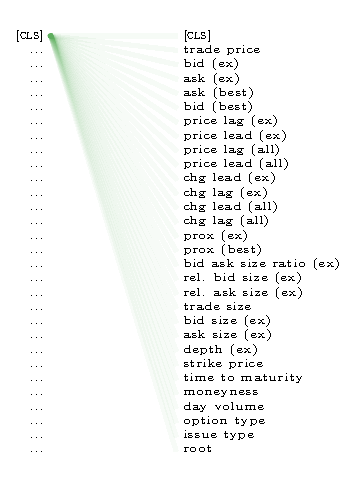
\includegraphics[width=.23\textwidth]{attention_head_1_layer_1_color_green_ise_quotes_mid.pdf}}\hfill
    \subfloat[Head (2,1)]{\label{sfig:ab}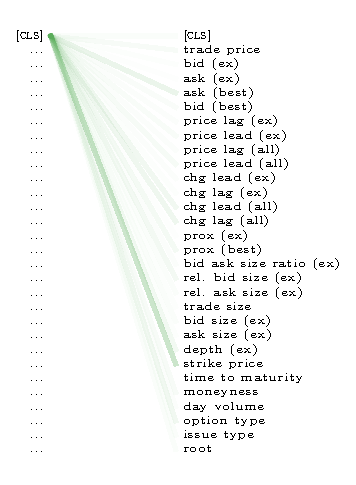
\includegraphics[width=.23\textwidth]{attention_head_1_layer_2_color_green_ise_quotes_mid.pdf}}\hfill
    \subfloat[Head (3,1)]{\label{sfig:ac}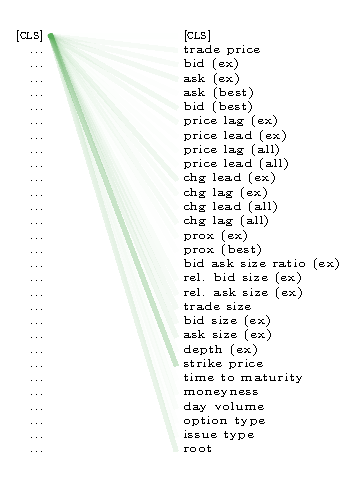
\includegraphics[width=.23\textwidth]{attention_head_1_layer_3_color_green_ise_quotes_mid.pdf}}\hfill
    \subfloat[Head (4,1)]{\label{sfig:ad}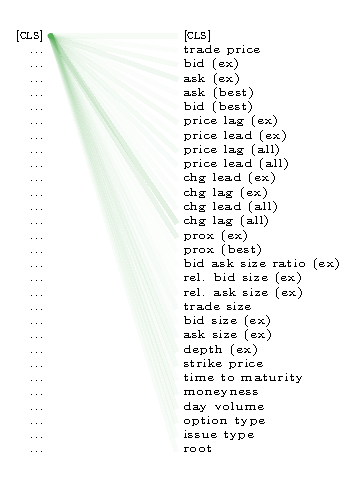
\includegraphics[width=.23\textwidth]{attention_head_1_layer_4_color_green_ise_quotes_mid.pdf}}\\
    % \subfloat[Head (1,2)]{\label{sfig:ba}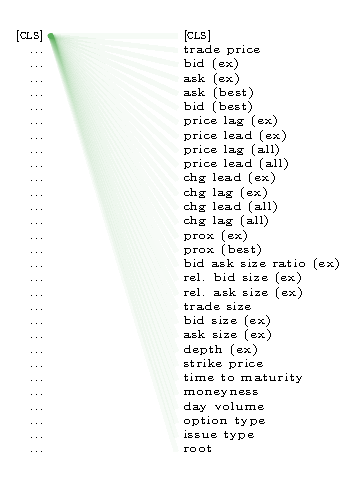
\includegraphics[width=.23\textwidth]{attention_head_2_layer_1_color_green_ise_quotes_mid.pdf}}\hfill
    % \subfloat[Head (2,2)]{\label{sfig:bb}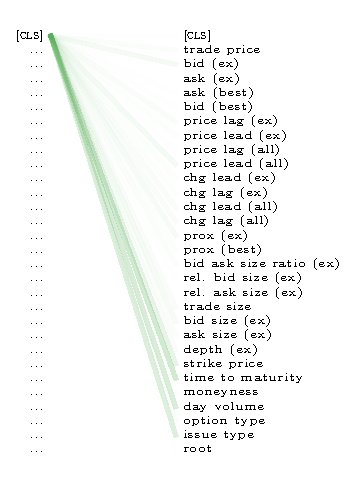
\includegraphics[width=.23\textwidth]{attention_head_2_layer_2_color_green_ise_quotes_mid.pdf}}\hfill
    % \subfloat[Head (3,2)]{\label{sfig:bc}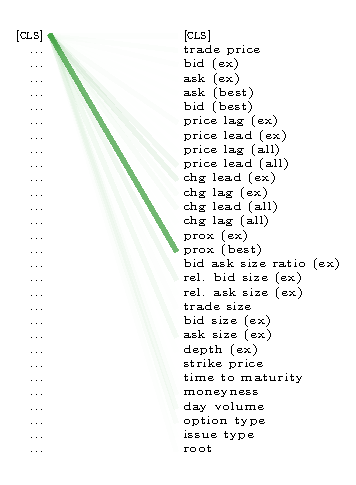
\includegraphics[width=.23\textwidth]{attention_head_2_layer_3_color_green_ise_quotes_mid.pdf}}\hfill
    % \subfloat[Head (4,2)]{\label{sfig:bd}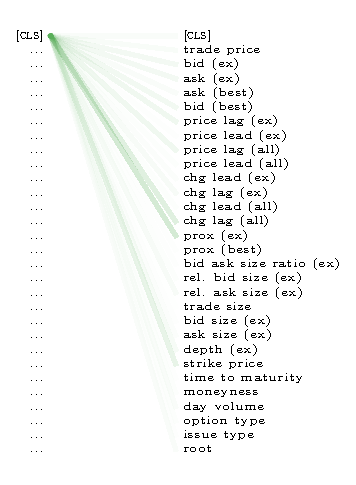
\includegraphics[width=.23\textwidth]{attention_head_3_layer_4_color_green_ise_quotes_mid.pdf}}\\
    % \subfloat[Head (1,3)]{\label{sfig:ca}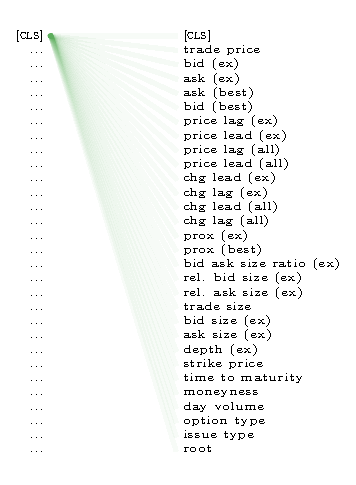
\includegraphics[width=.23\textwidth]{attention_head_3_layer_1_color_green_ise_quotes_mid.pdf}}\hfill
    % \subfloat[Head (2,3)]{\label{sfig:cb}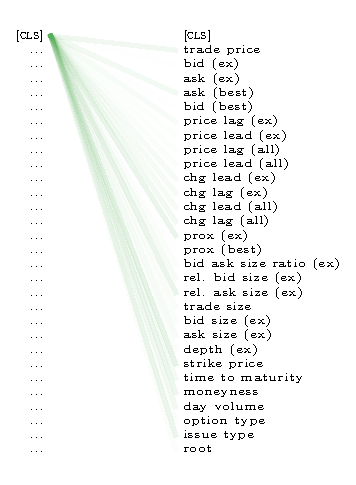
\includegraphics[width=.23\textwidth]{attention_head_3_layer_2_color_green_ise_quotes_mid.pdf}}\hfill
    % \subfloat[Head (3,3)]{\label{sfig:cc}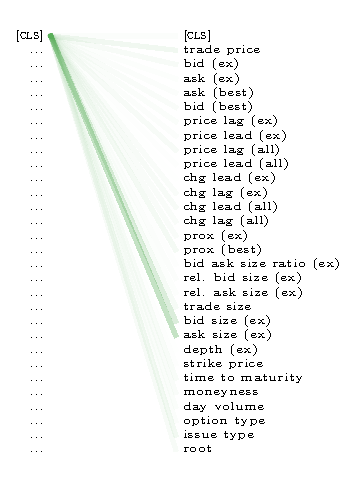
\includegraphics[width=.23\textwidth]{attention_head_3_layer_3_color_green_ise_quotes_mid.pdf}}\hfill
    % \subfloat[Head (4,3)]{\label{sfig:cd}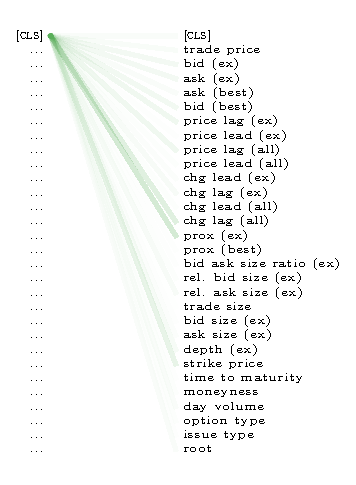
\includegraphics[width=.23\textwidth]{attention_head_3_layer_4_color_green_ise_quotes_mid.pdf}}\\
    % \subfloat[Head (1,4)]{\label{sfig:da}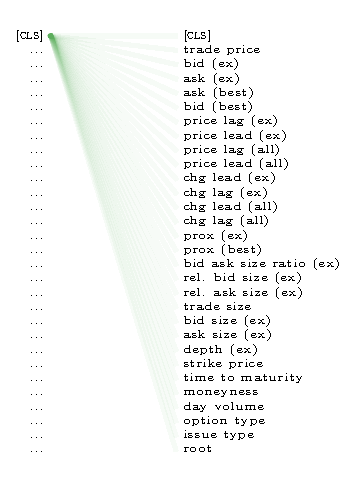
\includegraphics[width=.23\textwidth]{attention_head_4_layer_1_color_green_ise_quotes_mid.pdf}}\hfill
    % \subfloat[Head (2,4)]{\label{sfig:db}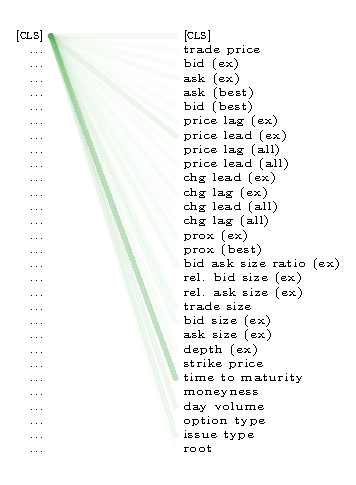
\includegraphics[width=.23\textwidth]{attention_head_4_layer_2_color_green_ise_quotes_mid.pdf}}\hfill
    % \subfloat[Head (3,4)]{\label{sfig:dc}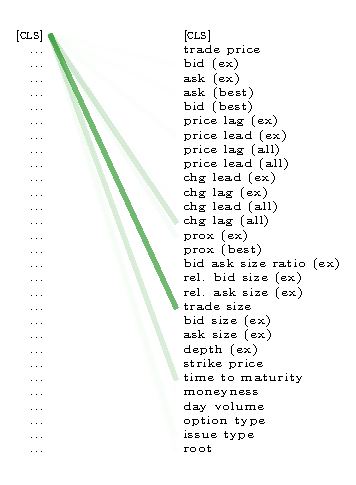
\includegraphics[width=.23\textwidth]{attention_head_4_layer_3_color_green_ise_quotes_mid.pdf}}\hfill
    % \subfloat[Head (4,4)]{\label{sfig:dd}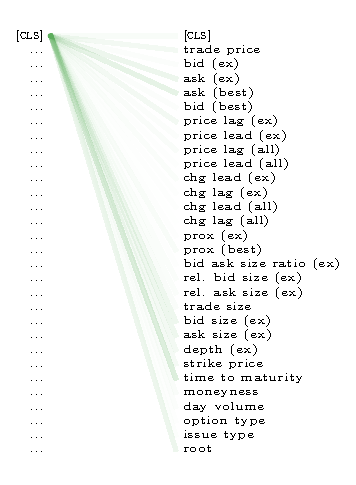
\includegraphics[width=.23\textwidth]{attention_head_4_layer_4_color_green_ise_quotes_mid.pdf}}\\
    % \subfloat[Head (1,5)]{\label{sfig:ea}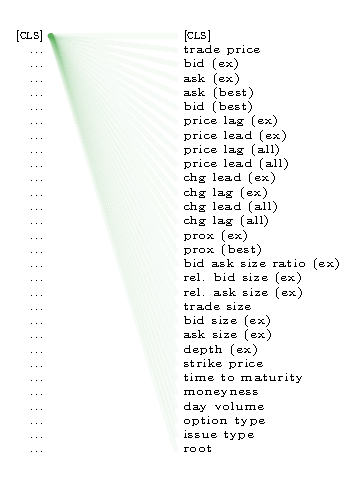
\includegraphics[width=.23\textwidth]{attention_head_5_layer_1_color_green_ise_quotes_mid.pdf}}\hfill
    % \subfloat[Head (2,5)]{\label{sfig:eb}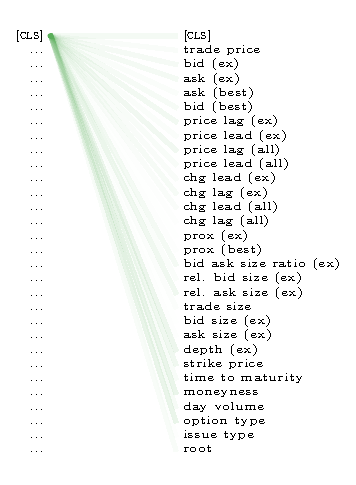
\includegraphics[width=.23\textwidth]{attention_head_5_layer_2_color_green_ise_quotes_mid.pdf}}\hfill
    % \subfloat[Head (3,5)]{\label{sfig:ec}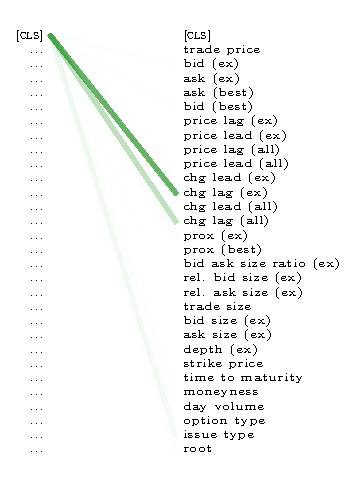
\includegraphics[width=.23\textwidth]{attention_head_5_layer_3_color_green_ise_quotes_mid.pdf}}\hfill
    % \subfloat[Head (4,5)]{\label{sfig:ed}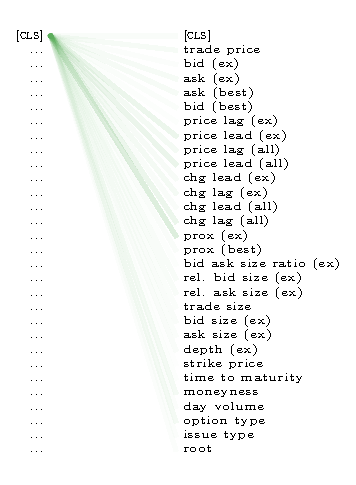
\includegraphics[width=.23\textwidth]{attention_head_5_layer_4_color_green_ise_quotes_mid.pdf}}\\
    % \subfloat[Head (1,6)]{\label{sfig:fa}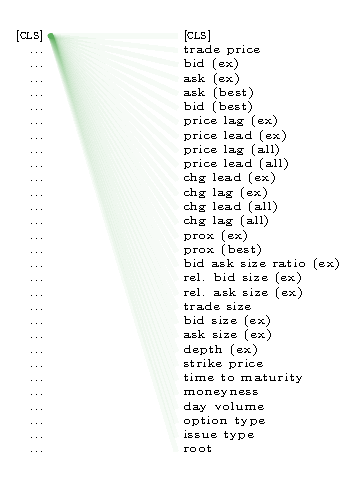
\includegraphics[width=.23\textwidth]{attention_head_6_layer_1_color_green_ise_quotes_mid.pdf}}\hfill
    % \subfloat[Head (2,6)]{\label{sfig:fb}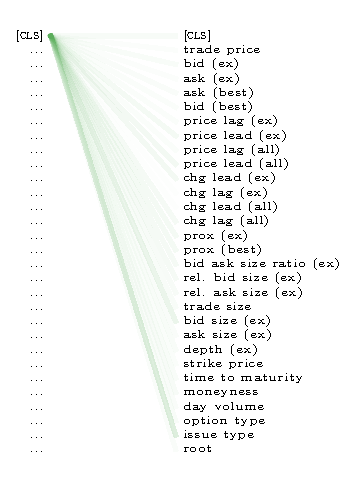
\includegraphics[width=.23\textwidth]{attention_head_6_layer_2_color_green_ise_quotes_mid.pdf}}\hfill
    % \subfloat[Head (3,6)]{\label{sfig:fc}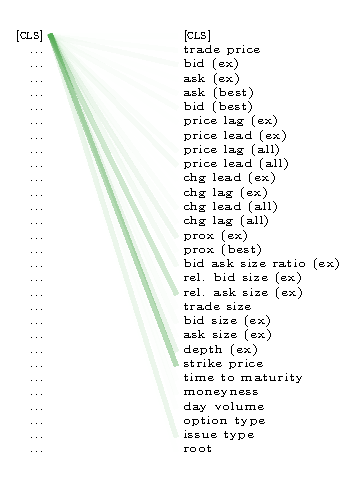
\includegraphics[width=.23\textwidth]{attention_head_6_layer_3_color_green_ise_quotes_mid.pdf}}\hfill
    % \subfloat[Head (4,6)]{\label{sfig:fd}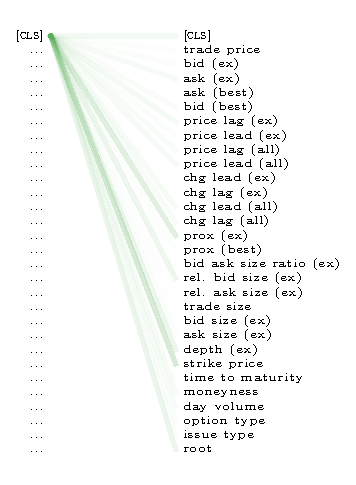
\includegraphics[width=.23\textwidth]{attention_head_6_layer_4_color_green_ise_quotes_mid.pdf}}\\
    % \subfloat[Head (1,7)]{\label{sfig:ga}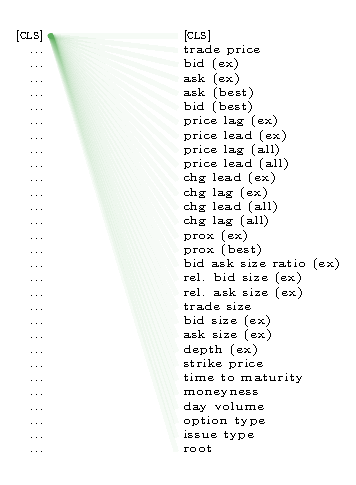
\includegraphics[width=.23\textwidth]{attention_head_7_layer_1_color_green_ise_quotes_mid.pdf}}\hfill
    % \subfloat[Head (2,7)]{\label{sfig:gb}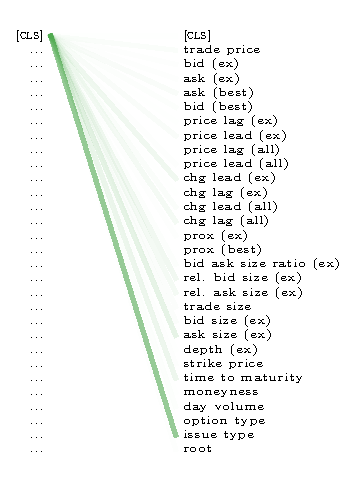
\includegraphics[width=.23\textwidth]{attention_head_7_layer_2_color_green_ise_quotes_mid.pdf}}\hfill
    % \subfloat[Head (3,7)]{\label{sfig:gc}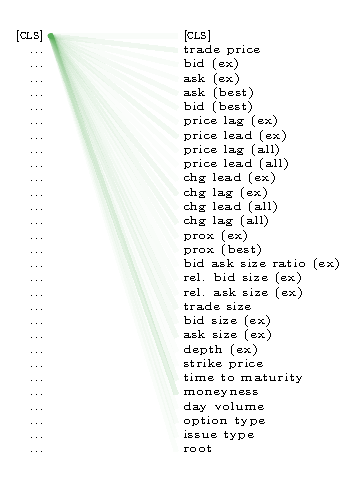
\includegraphics[width=.23\textwidth]{attention_head_7_layer_3_color_green_ise_quotes_mid.pdf}}\hfill
    % \subfloat[Head (4,7)]{\label{sfig:gd}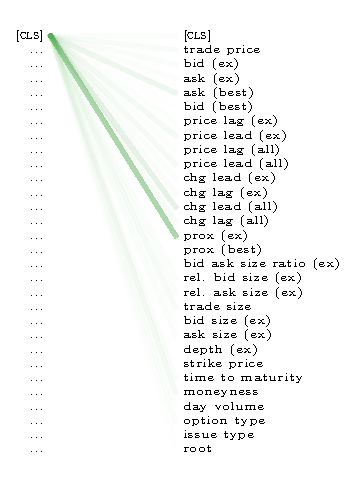
\includegraphics[width=.23\textwidth]{attention_head_7_layer_4_color_green_ise_quotes_mid.pdf}}\\
    % \subfloat[Head (1,8)]{\label{sfig:ha}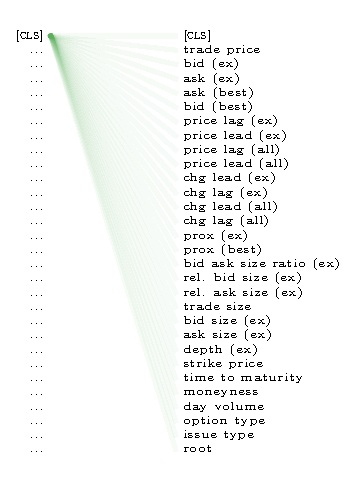
\includegraphics[width=.23\textwidth]{attention_head_8_layer_1_color_green_ise_quotes_mid.pdf}}\hfill
    % \subfloat[Head (2,8)]{\label{sfig:hb}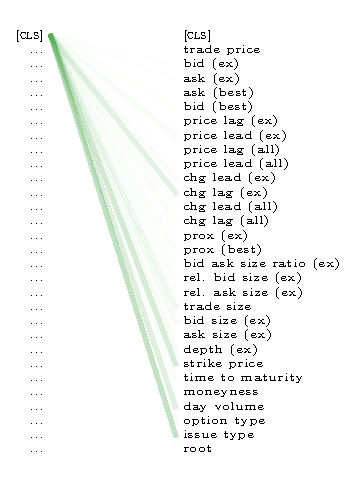
\includegraphics[width=.23\textwidth]{attention_head_8_layer_2_color_green_ise_quotes_mid.pdf}}\hfill
    % \subfloat[Head (3,8)]{\label{sfig:hc}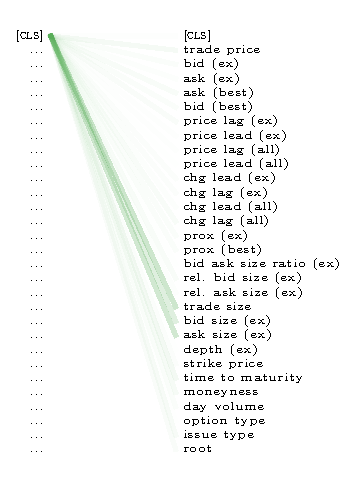
\includegraphics[width=.23\textwidth]{attention_head_8_layer_3_color_green_ise_quotes_mid.pdf}}\hfill
    % \subfloat[Head (4,8)]{\label{sfig:hd}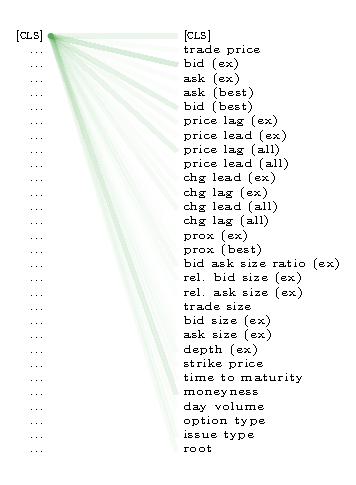
\includegraphics[width=.23\textwidth]{attention_head_8_layer_4_color_green_ise_quotes_mid.pdf}}\\
    \caption[Rule-Like Roles of All Attention Heads]{Attention heads that correspond to trade classification rules. Tuple denotes the location of the attention head in the model in the form of (layer, head). Plot visualizes the attention weights for a trade executed at the quote, correctly classified by the model.}
    \label{fig:attention-heads-ise-all-transformer}
\end{figure}